\subsection{Maximum Weight Spanning Tree}
\textbf{Input}: a connected, weighted, undirected graph $ G = (V , E) $ with weight function $ w : E \to R $. 

\textbf{Goal}: Find a maximum weight spanning tree in $G$. 

Because this is the problem of finding a maximum weight of maximum independent set in a graphic matroid, the greedy algorithm is optimal.

\subsection{Kruskal's Algorithm}
\textbf{Main Idea}: Sort the elements in the ground set (edges) in decreasing order of weight and then repeatedly add edge as long as adding new edge keeping the graph acyclic.

\textbf{Consider}: Suppose Kruskal's algorithm has found the following edges, what makes the algorithm to decide to pick an edge?

Think in a shallow way. The new edge shall not create a cycle in the graph. To be more specific, if the vertices from the new edge belongs to the same component then it will introduce a cycle since vertices with in the component are already connected. Conversely, if the vertices come from different components then it cannot be a cycle.

So Kruskal's algorithm maintain the connected components it has discovered so far then includes edge $ (u, v) $ lie in different component before the inclusion.

\textbf{Remark}: So far we have focused on finding maximum spanning tree but it turns out that the greedy algorithm works for finding minimum spanning tree as well. The only difference is to sort the weights by descending order for minimum spanning tree. For minimum spanning tree, we can use the same greedy algorithms.

\subsubsection{Algorithm}
Kruskal's algorithm finds a minimum weight spanning tree in a connected, weighted, undirected graph.
\begin{itemize}
	\item Sort and renumber the edges in increasing order of weight as $ e_1 , \dots, e_n $.
	\item Maintain a graph G with the same vertices as the original graph to track the edges chosen already.
	\item When considering $ e_i = (u, v) $, add $e_i$ to the graph if and only if $u$ and $v$ lie in different components. To do this, we need two routines.
	\begin{itemize}
		\item Find operation: return the component for a vertex $u$.
		\item Union operation: merge two components together.
	\end{itemize}
\end{itemize}
We define a \textsc{union\_find} data structure for find and union operation. Initially no edge is chosen by the algorithm and every vertex is a component by itself. Therefore, we will initialize the data structure to $n$ singleton components.

Now we are going to explore some of the possible data structure to be used for \textsc{union\_find}.

\paragraph{Attempt 0.} Maintain the information in array. Make index of array is the vertex name and value is the name of the component.

For this structure, find operation is $\mathcal{O}(1)$. Union(u, v) = $\mathcal{O}(n) $, since in worst case you may have to rename all the vertices. In the course of Kruskal's algorithm, $n-1$ union operations to perform. So this is a rather expensive design choice.

\paragraph{Attemp 1.} Suppose $u$'s set contains $n_1$ elements and $v$'s set contains $n_2$ elements. 

When Union-ing two sets, change the name for the elements in the \textbf{smaller} sets. But in the worst case, the union still takes $n$ steps. Moreover, even in a good case, there is only one element in a set but we still need to scan the whole list to know the size of set. Therefore, we introduce a new array to maintain a linked list for each set containing the elements in that set.

Remark: The array is used to from vertex to set and the linked list is used to find the vertices of each set.

Even with the help of new linked list, an individual union operation could still take $\Theta(n)$ steps. However, we can use \textbf{amortized analysis} to make the our analysis more tight by looking at the whole sequence instead of single operation. In fact, any \textbf{sequence} of $k$ union operations performed by Kruskal's algorithm take only $\mathcal{O}(k\log n)$ steps.

\subparagraph{Amortized Analysis.} In computer science, amortized analysis is a method for analyzing a given algorithm's complexity, or how much of a resource, especially time or memory, it takes to execute. The motivation for amortized analysis is that looking at the worst-case run time per operation, rather than per algorithm, can be too pessimistic. The target of amortized analysis is rather special since it is neither average nor worst case.

For example, suppose given two sets of vertices $A$ and $B$, the goal is to calculate the union of the sets. Also $|A| > |B|$, so the cost of operation is $|B| = n$.
 
Accounting method is used for analysis:
\begin{itemize}
	\item Set up an account for each element in the data structure. 
	\item Charge 1 to each element in the smaller set for a union operation. 
	\item Every time an element is charged. It joins a set at least twice as large. \\ $\rightarrow$No element is charged more than $\log n$ times.
\end{itemize}

Therefore, the total cost of a sequence of ($n-1$) union operations to union $A$ and $B$ is at most $n \log n$. (With some most carefully analysis, $k$ union cost at most $k\log k$. But $n\log n $ is good enough for the course.)

\paragraph{Attemp 2.} Maintain connected components in a tree so that we have a forest as follows. The name of the component is the element at the root. The name of each vertices are saved in the array of leaves. For each leaf in the tree, keep a pointer to its parent. 

\begin{figure}[H]
	\centering
	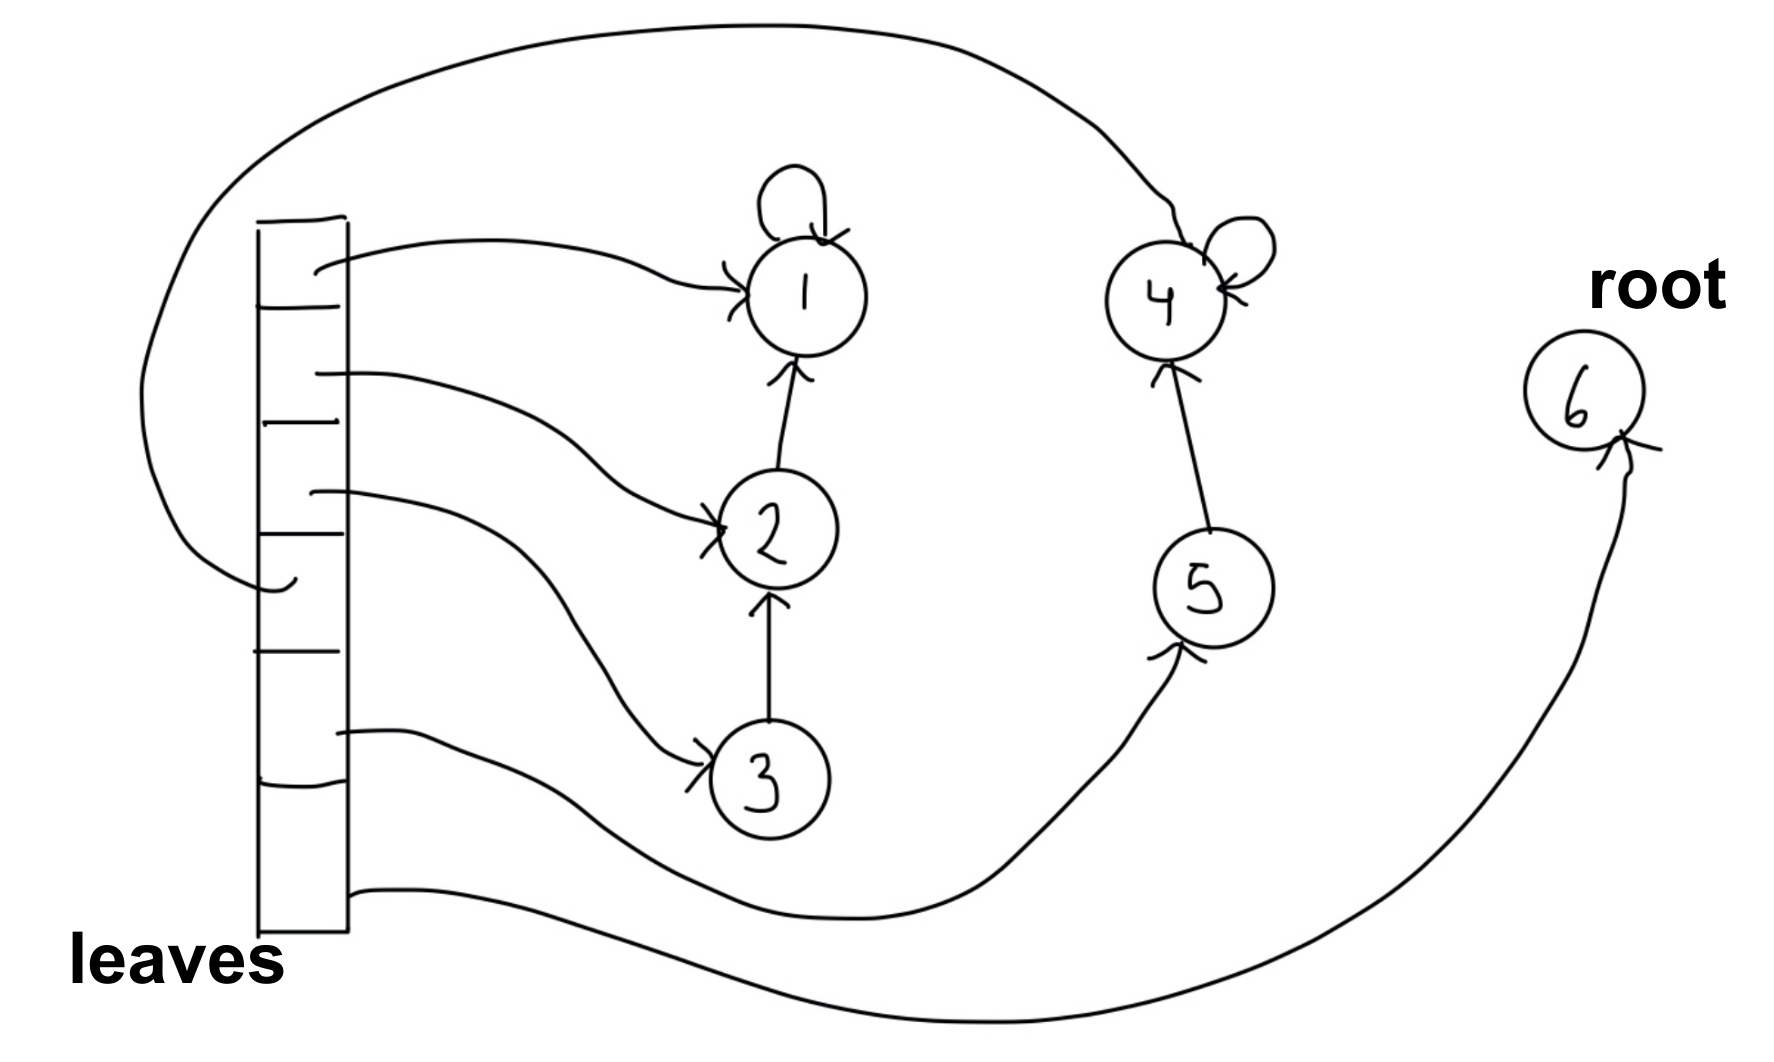
\includegraphics[width=0.5\textwidth]{attemp-2.png}
\end{figure}

\subparagraph{\textsc{Find}.} Traverse up the tree by the pointer until you find the end of linked list, which is a root and you will have found the component of the vertex. Hence, \textsc{Find} cost a proportion of the height of the tree. 

\subparagraph{\textsc{Union}.} \textsc{Union} make one root point to the other. 
%Make the root of the tree with pure elements prompt up to the root of the other tree. 

How to find the time complexity of each operation? We can do the same optimization trick like in Amortized Analysis. We make the root of the smaller tree point to the root of the larger tree. Based on that, we claim that all tree heights at all times are $ O(\log n) $.
\begin{claimproof}
	Think about any element in any of the trees, when the cost for it passes through the root increase by 1? After the tree unions with other tree, in which case the size of the sets increases at least by twice. Therefore, no element can be more than $O(\log n)$ away from the root.
\end{claimproof}

Therefore, we have the confidence to claim that \textsc{Find} operations are $ O(\log n) $ in the worst-case. The \textsc{Union} operations of arbitrary pairs of elements are also $ O(\log n) $.

Recall that $|E| = m$ and $|V| = n$. Kruskal's algorithm does $O(m)$ find operations and $O(n)$ union operations. So overall, $O(m \log n)$ steps for all union and find operations. Note that sorting edges at the beginning already takes $O(n\log n)$ steps. (? Here it should be $O(m\log m)$, but $O(m\log m) = O(n\log n)$?) So far \textsc{union\_find} is not the sole bottleneck since it has the same time complexity with sorting. 

But still, there is one more optimization for \textsc{Union} operation even though it will not help to improve the overall performance of Kruskal's algorithm.

\paragraph{Path Compression.}
First, let's reflect on one of the features of the tree we just build. 

Unlike with the common tree structures, here we start from any internal node pointing by the pointer and then go upward from the child to its parent. 

In the common tree (binary search tree, heap tree), we have to limit the number of children because it will cause the traversal order problem and increase the complexity of the problem.

By controversial, the path in our bottom has deterministic direction. Moreover, like always, the height of the tree is the number of operations for solving problem. Therefore, we would keep the tree as much bushy and short as possible to reduce the number of operations.

Now motivated by making the tree bushy and short, we can do path compression as follows:

When doing \textsc{find}($u$), for each node encountered on the path from leaf $u$ to the root, make it a child of the root.

Note that path compression could not improve the worst case time of either \textsc{find} or \textsc{union}. But it gives a great amortized complexity. Any sequence of $m$ starting from the initial \textsc{union-find} data structure on elements takes at most $O(m\log^*n)$ time.
\begin{definition}
	$\log^*n$ is a really really slow function which almost like a constant. It is the number of times you need to take $\log$ to get $n$.
\end{definition}
For example. $\log^* 16 = 3$. $\log^* (2^{16} = 65536) = 4$. $\log^* (2^{65576} = 65536) = 4$

We did not cover the analysis of path compression during class.
\subsection{Prim's Algorithm}
Prim's algorithm is another greedy algorithm for finding a maximum weight spanning tree. In the canonical greedy algorithm, we keep adding edge one at a time but how to select the right edge in the graph? Here we introduce a concept \textbf{cut.}

\begin{definition}
	A \textbf{cut} in a graph $G = (V, E)$ is defined by non-trivial partition $ V_1 \cup V_2 $ of $V$. The cut $ (V_1, V_2) $ is a set of edges that have exactly one end point in $ V_1 $.
\end{definition}

\begin{claim}
	For $e \in \text{cut}(S, V-S)$, if $e$ is the heaviest edge in the set. Then it will not cause a cycle with other edges have been connected by greedy algorithm. Therefore $e$ will be included in the maximum weighted independent set.
\end{claim}
\begin{claimproof}
	By the canonical greedy algorithm, we consider edges in decreasing order of weights. By the time we consider the edge $e$, we have not consider any other edge cross the two sets of the cut yet since $e$ has the largest weight. Therefore, $e$ will not cause any cycle with the edges that the greedy algorithm has chosen. Because you need two edges cross the two components to get a cycle.
\end{claimproof}

Prim's algorithm is one specialization of this idea that if you can find the heaviest edge in each cut then you can build a minimum spanning tree. Prim's algorithm consider a particular set of cuts.

\textbf{Main Idea}: Split the graph into two sets $S$ and $V-S$. Some vertex $s$ is arbitrarily chosen as the initialization of $S$. First consider the cuts consisting $s$. Find the cheapest edge $(s, v)$. Bring $v$ into set $S$. Repeat the steps for the next heaviest cutting edge.

\subsection{Algorithm}
Initially, 
\[
d(v) = 
\begin{cases}
w(s, v) \text{, if $(s,v) \in E$}\\
\infty \text{, otherwise}
\end{cases}
\]
For each $ y \in V-S $, maintain $ d(y) $, which is the weight of the lightest edge $(x, y)$ from $V-S$ to any source vertex $x$ in $S$.

At each iteration, when we move the vertex $y$ that has the cheapest
edge to a vertex in $S$, we need to update every neighbor $v$ of $y$ so that $ d(v) = \min(d(v), w(v, y)) $.
\begin{figure}[H]
	\centering
	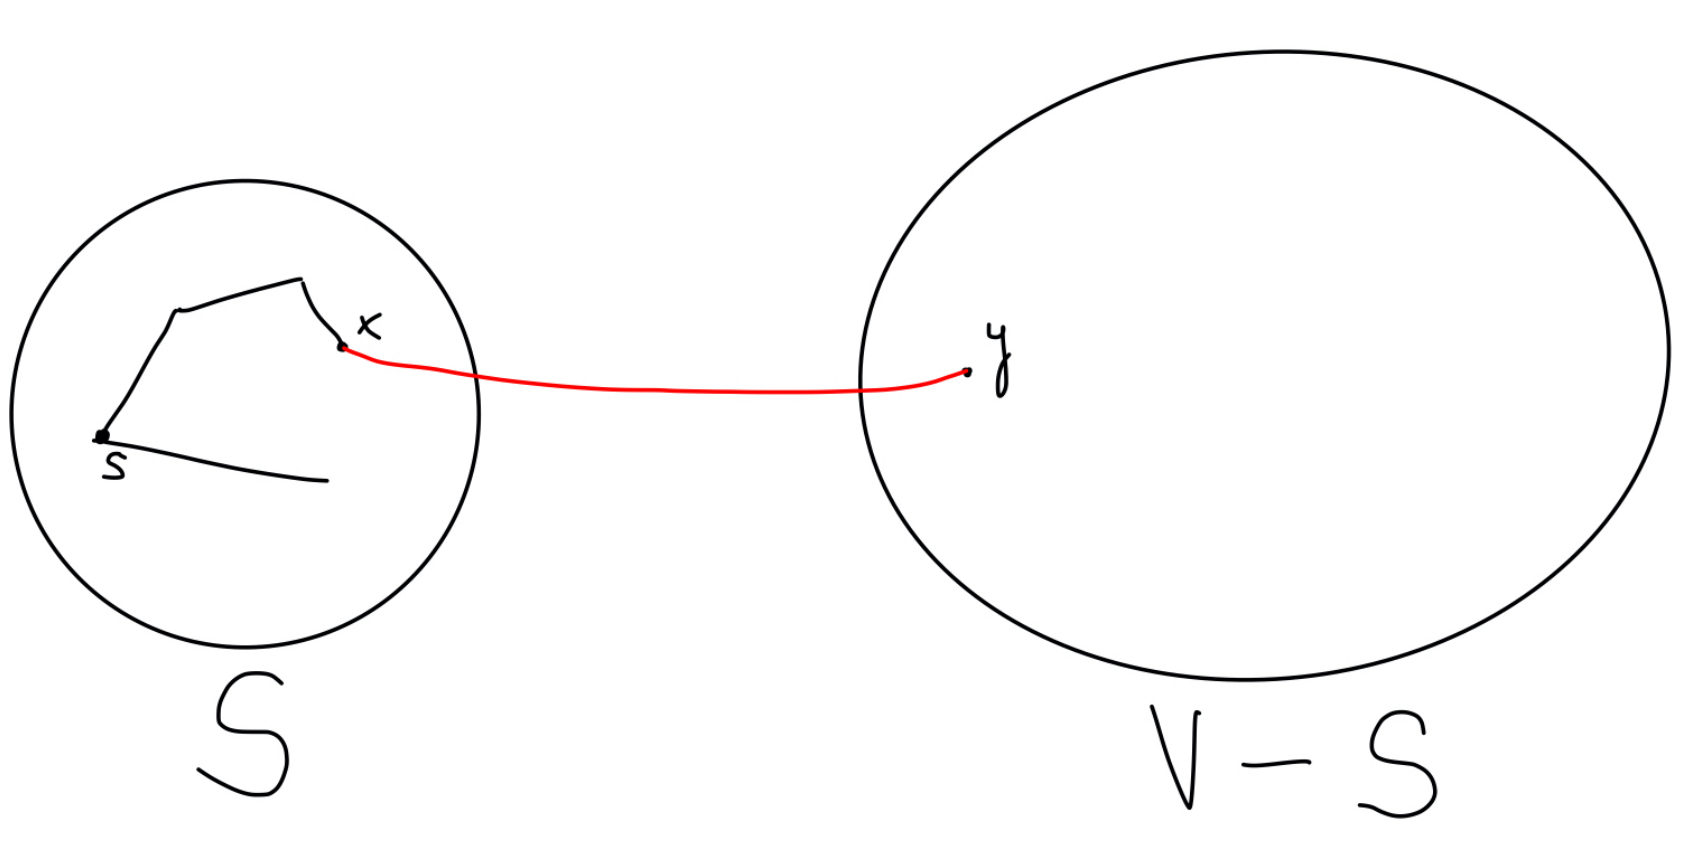
\includegraphics[width=0.5\textwidth]{prim.png}
\end{figure}

\subsection{Time Complexity}
If we maintain the $ d(v) $s in an array $ A $, the complexity is $ O(n^2) $ because we need to first find the minimum in $A$, and once we've found the minimum we need to update all the neighbors of the minimum.

If we maintain the $ d(v) $s in a min-heap, the complexity is $ O(m log(n)) $. Usually $m \le n$.

















